	\documentclass[10pt,oneside]{CBFT_book}
	% Algunos paquetes
	\usepackage{amssymb}
	\usepackage{amsmath}
	\usepackage{graphicx}
	\usepackage{libertine}
% 	\usepackage[bold-style=TeX]{unicode-math}
	\usepackage{lipsum}

	\usepackage{natbib}
	\setcitestyle{square}

	\usepackage{polyglossia}
	\setdefaultlanguage{spanish}


	\usepackage{CBFT.estilo} % Cargo la hoja de estilo

	% Tipografías
	% \setromanfont[Mapping=tex-text]{Linux Libertine O}
	% \setsansfont[Mapping=tex-text]{DejaVu Sans}
	% \setmonofont[Mapping=tex-text]{DejaVu Sans Mono}

	%===================================================================
	%	DOCUMENTO PROPIAMENTE DICHO
	%===================================================================

\begin{document}

\chapter{Transformaciones canónicas}

% =================================================================================================
\section{Funciones generatrices}
% =================================================================================================

Consideraremos ahora varios casos diferentes de dependencia en la función generatriz,
\[
	F_1 = F_1(q_i,Q_i,t)
\]
\[
	\sum p_i \dot{q}_i - H + K - \sum P_i \dot{Q}_i - \dpar{F_1}{q_i} \dot{q}_i - \dpar{F_1}{Q_i} \dot{Q}_i -
	\dpar{F_1}{t} = 0 
\]
\[
	\sum \left( p_i - \dpar{F_1}{q_i} \right) \dot{q}_i  - \sum \left( P_i + \dpar{F_1}{Q_i} \right) \dot{Q}_i -
	\dpar{F_1}{t} - H + K = 0 
\]
y la transformación canónica queda definida por 
\[
	\dpar{F_1}{q_i} = p_i \qquad \qquad \dpar{F_1}{Q_i} = - P_i \qquad \qquad \dpar{F_1}{t} = K-H
\]

Todas las combinaciones posibles son 
\[
	F_1 = F_1(q_i,Q_i,t) \qquad 
	F_2 = F_2(q_i,P_i,t) \qquad 
	F_3 = F_3(p_i,Q_i,t) \qquad 
	F_4 = F_4(p_i,P_i,t)
\]
y para $F_2$, por ejemplo, se tiene 
\[
	F_2(q_i,P_i,t) = \sum_i^N q_i P_i
\]
la cual es una identidad (transformación). Y
\[
	\dpar{F_2}{q_i} = P_i = p_i \qquad \dpar{F_2}{Q_i} = q_i = Q_i
\]

% =================================================================================================
\section{Algunos ejemplos de generatrices y transformaciones}
% =================================================================================================

La generatriz identidad
\[
	F_2(q_i,P_i) = \sum_i q_i P_i,
\]
es tal que las coordenadas y los momentos son los mismos (no cambian).
\[
	\dpar{F_2}{q_\ell} = P_\ell = p_\ell \qquad \qquad \dpar{F_2}{P_\ell} = q_\ell = Q_\ell
\]

La generatriz
\[
	F_1(q_i,P_i) = \sum_i q_i Q_i,
\]
tranforma coordenada en momento y viceversa, de manera que 
\[
	\dpar{F_1}{q_\ell} = Q_\ell = p_\ell \qquad \qquad \dpar{F_1}{Q_\ell} = -P_\ell = q_\ell
\]

Una rotación es una transformación canónica.
Otro nombre de las transformaciones canónicas es el de transformaciones de contacto.
Los pasajes de coordenadas usuales son casos de transformaciones canónicas.

% =================================================================================================
\section{Corchetes de Poisson}
% =================================================================================================

Sea $A=A(q_i,p_i,t)$ entonces
\[
	\frac{d}{dt}A = \sum_i \dpar{A}{q_i} \dpar{q_i}{t} + \dpar{A}{p_i} \dpar{p_i}{t} + \dpar{A}{t}
\]
y utilizando las ecuaciones canónicas
\[
	\frac{d}{dt}A = \underbrace{\sum_i \dpar{A}{q_i} \dpar{H}{p_i} - \dpar{A}{p_i} \dpar{H}{q_i}}_{\equiv [A,H]} + 
\dpar{A}{t}
\]
donde la sumatoria particular resultante se define como el corchete de Poisson.
Entonces
\[
	\frac{d}{dt}A = [A,H] + \dpar{A}{t}.
\]

Las constantes de movimiento en un sistema mecánico cumplen que su corchete de Poisson con el hamiltoniano es nulo.
\[
	\dpar{H}{p_i} = \dot{q}_i = [q_i,H] \qquad  -\dpar{H}{q_i} = \dot{p}_i = [p_i,H]
\]
Todas las {\it cosas} constantes en el tiempo en un sistema mecánico (no depende explícitamente del tiempo) deben
ser tales que su variación temporal sea el corchete de Poisson con el hamiltoniano.

Tendremos entonces, siguiendo la mecánica, que:
\[
	\dot{q}_i = [q_i,H] = \dpar{H}{p_\ell} \qquad \dot{p}_i = [p_i,H] = -\dpar{H}{q_\ell}
\]
que es otra manera de escribir las ecuaciones canónicas.
Si transformamos coordenadas llegaremos a 
\[
	\dot{Q}_i = [ Q_i, K ] \qquad \dot{P}_i = [ P_i, K ]
\]
junto con los corchetes fundamentales:
\[
	[p_i,q_j] = \delta_{ij} \qquad [p_i,p_j] = 0 \qquad [q_i,q_j] = 0
\]
de modo que el corchete entre los momentos es nulo así también como el corchete entre las coordenadas.

Si las variables son canónicas, satisfacen estos corchetes fundamentales para las nuevas $\{p,q\}$
\[
	[B,A] = \nabla_\xi B^t J \nabla_\xi A
\]

Si consigo un sistema mecánico y lo arreglo de modo que las coordenadas y momentos satisfagan 
\[
	[B_k, H ] = 0 \qquad \qquad  [B_k, B_\ell ] = 0 \forall k,\ell
\]
que significa que los momentos son constantes de movimiento y que entre sí tienen corchete nulo, entonces
existe una transformación canónica con todas las coordendas cíclicas.

Así, por ejemplo, $H,\ell^2, \ell_z$ tienen corchete nulo entre sí. Pero $\ell_x, \ell_y, \ell_z$ no tienen corchete nulo
entre sí; no puedo armarme una transformación canónica que me lleva a un espacio donde $\ell_x, \ell_y, \ell_z$ son
momentos generalizados.
Esto es similar a lo que ocurría con el CCOC de mecánica cuántica.


\begin{ejemplo}{\bf Moneda que desliza por un plano (sin gravedad)}

\notamargen{Ya se habló de este problema en la sección 2, con respecto a multiplicadores de Lagrange.}

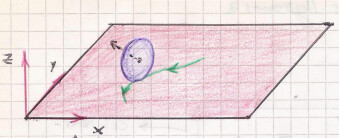
\includegraphics[scale=0.4]{images/fig_mc_moneda_dos_1.jpg}

El lagrangiano se puede escribir
\[
	\Lag = T = \frac 1 2 M V_{cm}^2 + \frac 1 2 I_3 \dot{\chi}^2 + \frac 1 2 I_3 \dot{\vp}^2
\]
y la velocidad del centro de masa es
\[
	\vb{V}_{cm} = - \vb{\Omega} \times \vb{x}
\]
y los $x_{cm}, y_{cm}$ no se pueden despejar en función de los ángulos de Euler.

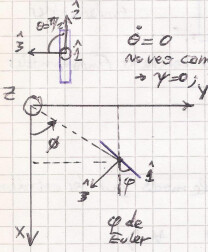
\includegraphics[scale=0.4]{images/fig_mc_moneda_dos_2.jpg}

\end{ejemplo}





% \bibliographystyle{CBFT-apa-good}	% (uses file "apa-good.bst")
% \bibliography{CBFT.Referencias} % La base de datos bibliográfica

\end{document}
